\chapter{A Framework for Automated Monitoring and Scaling of the SMACK Stack}
\label{ch:implementation}

This section gives a detailed view of the actual contribution in the scope of this thesis.
The developed applications, stress tests and tools are introduced and their architecture is illustrated.
To review the code, there is a public git repository containing the implementations mentioned in this chapter \footnote{https://bitbucket.org/B3n3/smack}.\\
For the development mainly the Java programming language was chosen, as it is platform independent and appeals a broad audience.

\section{The SMACK Monitoring Metrics and Elasticity Actions}
As part of the theoretical background, this section gives an overview of which metrics are considered as interesting for the context of this thesis.\\

\subsection{Kafka}
In the official DataDog Github repository there is a documentation of which metrics can be interesting when analyzing Kafka via JMX \cite{datadog_kafka}.
Those proposed metrics were considered and then refined by empirical experiments to find out which ones are good indicators when Kafka is under heavy load.\\
In Table~\ref{tab:jmx_kafka} the metrics considered in this thesis concerning Kafka monitoring are illustrated in detail.

\subsection{Cassandra}
DataDog also provides an introduction to Cassandra monitoring and emphasized which JMX values to investigate when monitoring a cluster \cite{datadog_cassandra}.
Like for the Kafka metrics, those presented MBeans were refined during empirical experiments.
In Table~\ref{tab:jmx_cassandra} all relevant Cassandra JMX metrics are listed and described.

\subsection{Spark}
During the analysis of the IoT application introduced earlier, all available JMX metrics are collected.
The script to extract the Spark JMX values of Section~\ref{sec:jmx_extract_tool} filters out everything which is not directly related to the driver running in Spark.
This is done by applying a regular expression as matching criteria, which looks like this: \verb"KafkaToCassandra|.driver", where \textit{KafkaToCassandra} is the Spark driver name in the IoT application.
The regular expression considers everything which is either part of the custom class or the driver itself.\\
It is necessary to use this approach, as the MBean names exposed by Spark contain IDs which change every time the driver is launched.
An example for such a name could be this: \textit{metrics:name=43f6de33-9485-4bbe-8dbf-263b62d2a15a-0005-driver-20170731143634-0001.driver.DAGScheduler.messageProcessingTime}.\\
By analyzing the plots of the collected metrics, the ones described in Table~\ref{tab:jmx_spark} are considered most interesting.

\subsection{Akka}
As mentioned in Section~\ref{sec:jmx_extract_tool}, Akka does not provide JMX metrics out of the box.
It is up to the developer to collect metrics and then implement the exposure of them.
In the course of the contribution of this thesis, those features are implemented.\\

Fortunately there is an open-source project to ease the task of exposing JMX values.
The framework is called \textit{Kamon}, which "is distributed as a core module with all the metric recording and trace manipulation APIs and optional modules that provide bytecode instrumentation and/or reporting capabilities" \cite{kamon}.\\
In addition there are two dedicated Akka modules in Kamon, which expose some useful default metrics.
To be able grab and expose JMX values from an existing application, AspectJ Weaver is used.
It is a non-trivial task to handle all required dependencies and correctly launch the application with AspectJ in a Docker container.
Setting up things require knowledge in the field of virtualisation with Docker and dependency management.\\

In addition to the already by Kamon provided metrics, \textit{KB/s} and \textit{Messages/s} are added to give more flexibility when monitoring the application.
In Table~\ref{tab:jmx_akka}, all considered metrics are illustrated and described in detail.


\subsection{Mesos}
As there is no possibility to enlarge RAM or CPU resources for Mesos and because it is the underlying system, there is no need to monitor it explicitly in the context of this thesis.


\section{Framework for Automated Monitoring and Scaling}
This section introduces the framework developed in the course of this thesis.
First there is an architecture overview to better understand how the respective components interact.
Secondly the respective components and tools are illustrated and explained in detail.

\subsection{Framework Architecture Overview}
In this section, an overview of the framework is given, including architecture and deployment diagrams.

\begin{itemize}
    \item \textbf{Automated Scaling Tool for SMACK}\\
          The scaling tool evaluates the collected metrics from the REST service and scales up or down the individual parts of the SMACK stack.
    \item \textbf{REST Service Collecting Monitoring Information}\\
          This is the service which collects all the extracted metrics and compiles them into a useful format.
          In addition there is the possibility to generate plots at runtime.
    \item \textbf{JMX Extraction Tool}\\
          This tool is designed to automatically extract interesting metrics from SMACK components via JMX and sending them to a central service, in this case the REST monitoring service.
    \item \textbf{Framework to Easily Launch SMACK in AWS}\\
          With the help of this framework it takes just a few command line calls to launch and deploy the whole SMACK stack in the cloud.
    \item \textbf{Deployment Blueprints}\\
          Those reference architecture and configuration recommendations help to launch the SMACK stack and getting most out of the available resource.
\end{itemize}

Figure~\ref{fig:architecture} illustrates the target architecture of the framework and how the tools and services interact with each other, while Figure~\ref{fig:overall_view} shows the deployment view.\\
The SMACK stack is the central element in this architecture and is illustrated by many AWS EC2 instances working together as one stack.
In the same environment - namely DC/OS - the JMX Extraction tool is running in Docker containers, collecting metric statistics from the SMACK stack.
For each node, or EC2 instance, there is exactly one Docker container started and associated.
The container runs on the same instance to be able to access the JMX values from the available services.\\

In case there is no service deployed on the node, the JMX extraction tool is idle and automatically starts extracting as a service gets deployed.\\
To launch and setup DC/OS the Cloud Formation tool of AWS is used, which manages the complex installation of all required components and glues them together automatically.\\
The extracted metric values are directly send to the REST monitoring service, which runs on its own dedicated EC2 instance totally independent of the DC/OS setup.
There the information is collected and combined to be evaluated later.\\

If it is the case that the IOT application is running in the SMACK stack, the load generator introduced in section \ref{sec:load_generator} is also part of the setup.
As described, the AWS EC2 Container Service is used to easily orchestrate the execution of multiple docker images performing the requests.
ECS enables to simply de- or increase the amount of running Docker containers and is also independent of the DC/OS setup.
There is no information flow from DC/OS to the load generator.\\

All previously described parts of the setup are running in the AWS cloud.
The only application running on a local machine is the scaling tool itself.
By querying the REST monitor, the scaling tool gets up-to-date information about the workload of the SMACK stack.
In case the stack get's offline or does not respond in time, the monitoring service is still responsive because it is completely decoupled from the rest of the stack.
The user interacts with the scaling tool which in turn interacts directly with DC/OS to manipulate the SMACK stack in case a component needs to be scaled up or down.

\begin{figure}[!htbp]
  \centering
  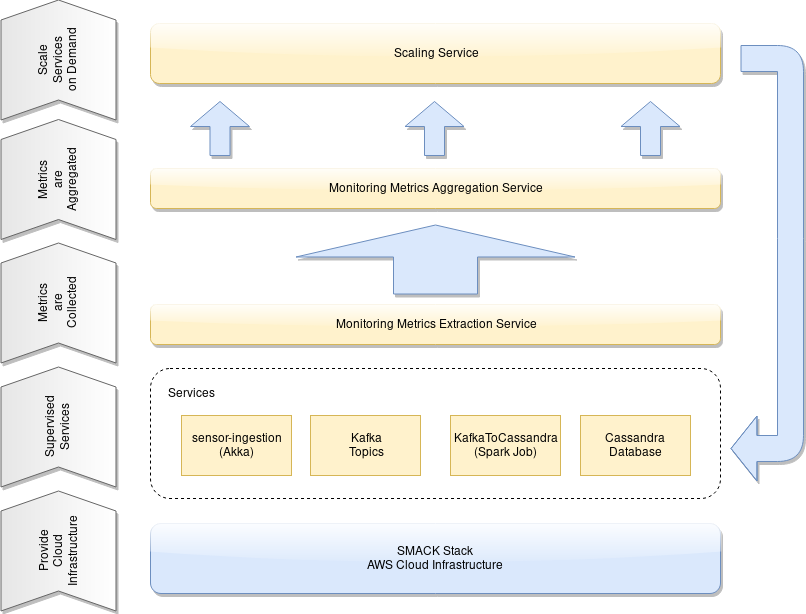
\includegraphics[keepaspectratio=true,scale=0.55]{img/architecture}
    \caption{Framework Target Architecture}
    \label{fig:architecture}
\end{figure}

\begin{figure}[!htbp]
  \centering
  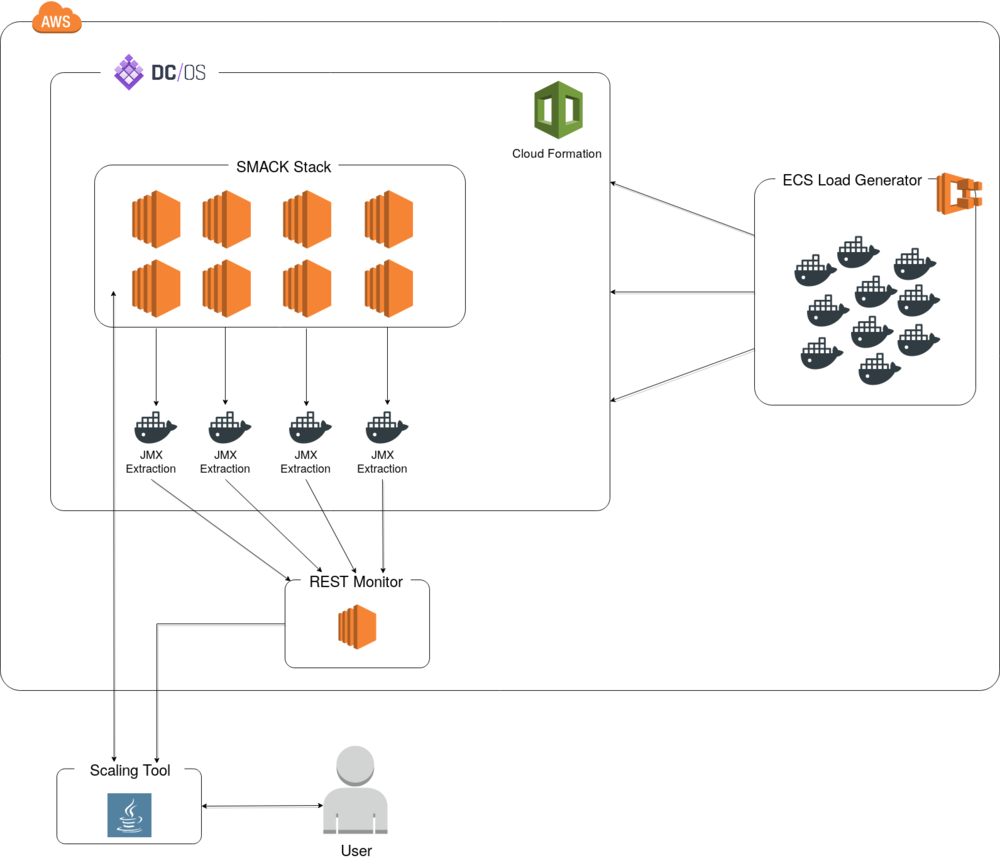
\includegraphics[keepaspectratio=true,scale=0.47]{img/overall_view}
    \caption{Framework Deployment View}
    \label{fig:overall_view}
\end{figure}



\subsection{Monitoring Metrics Extraction Service}
\label{sec:jmx_extract_tool}

To be able to monitor each SMACK component individually, considering more than just plain RAM and CPU usage, a more sophisticated approach is required than only observing the provided DC/OS usage metrics.\\
First we will have a look on the technical aspect of how to gather information and then why the proposed approach was chosen.\\

Collecting runtime information from an application is a common task and there are some well-known ways to do so.
Webservices for example, often provide a REST API to access internal status information.
As the applications used in this thesis all run in the Java Virtual Machine (JVM), it is possible to use the Java Management Extensions (JMX) as information channel.\\
This is especially useful as Kafka, Cassandra and Spark are configurable to publish monitoring statistics via JMX without any extra programming.
Akka is not able by default to export to JMX which means all the steps - form acquiring the statistical data to publishing them - have to be programmed into the Akka application.\\

Figure~\ref{fig:jmx} shows the basic architecture of JMX.
The distributed services level, serves as entry point to access the interface.
There is no defined specification and the purpose is to provide a way to communicate with the deeper agent level.\\
Through the interface the client is able to access the agent level, where the agents reside and are responsible for the communication with the instrumentation level.
In the last level, the real resources can be found, which are managed and configured with the so called \textit{Managed Beans (MBeans)}.\\
With the help of MBeans it is possible for an application to expose values through JMX, which can then be read by a client via the JMX interface.\\

\begin{figure}[!htbp]
  \centering
  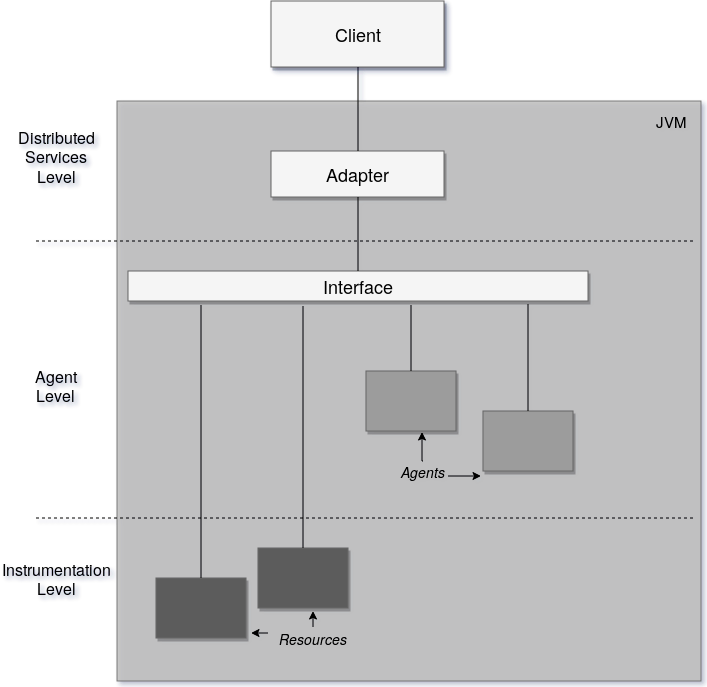
\includegraphics[keepaspectratio=true,scale=0.45]{img/jmx}
    \caption{JMX Architecture Overview}
  \label{fig:jmx}
\end{figure}

In order to access JMX MBean values of running JVM instances, there are some open source tools available.
JConsole is a graphical tool which ships with the JDK and allows the user to get an overview of a running system.
However, this tool requires a GUI, and does not provide an API to use it with scripts or via command line.\\
An open-source tool, which offers this interface is Jmxterm.
"Jmxterm is a command line based interactive JMX client.
It's designed to allow user to access a Java MBean server in command line without graphical environment.
In another word, it's a command line based jconsole" \cite{jmxterm}.\\
MBeans contain attributes which could be \textit{Value}, \textit{OneMinuteRate}, \textit{Mean}, \textit{Count} and so on.
As part of the contribution of this thesis, a script to automatically extract the desired MBean values and send them to a monitoring service is provided.
The abstract algorithm of the script can be described as follows:

\begin{enumerate}
    \item Get the current timestamp.
    \label{enum:current}
    \item Read the provided JMX commands from the input file.
    \item Create a list of all occurring MBeans in the given file.\\
        This list is needed, as the output of Jmxterm does not contain the name of the MBean itself.
    \item Open the CSV output file and add a column header if the file is empty.
    \item Execute Jmxterm with the provided command file and split the output lines by newline.
    \item For each line:
        \begin{enumerate}
            \item Extract the attribute name and the respective value of the output.
            \item Write the data into the CSV file.
            \item Send the data to the given REST monitoring service via HTTP POST.
        \end{enumerate}
    \item Close all files and sleep for a given period of time.
    \item Go to \ref{enum:current}.
\end{enumerate}

The exported values of the script are: \textit{Timestamp}, \textit{MBean name}, \textit{Attribute name}, \textit{Value} and \textit{Hostname}.\\
The hostname is important, as it is the only way to distinguish from which node the value comes from.
In addition it is required to later on generate statistics and accumulate the value of the same MBean-Attribute combination across different nodes.\\
The script works fine for a static input file, which means the names of the MBeans are known in advance and do not change during the analysis.
However, Spark exposes MBeans which contain the ID of the worker node or the task number.
This makes it impossible to predefine a list of MBean names which the script should observe and send to the monitoring service.
Because of this problem, another script is implemented to extract interesting MBean names from Sparks JMX view.\\
An abstract overview of how the script works could be the following:

\begin{enumerate}
    \item Open the connection to Sparks JMX.
    \item Store all available MBeans inclusive their attributes in a list.
    \item Go through the list and filter out only interesting ones (with a regular expression).
    \item Extract the name of the attributes to the respective MBean.
    \item Store the Jmxterm commands to get the values of an MBean attribute into a command file.
\end{enumerate}

In order to be able to automatically generate new Spark command files during runtime, the script is executed regularly by the JMX extraction script.
This enables the setup to simply launch the extractor without having to deal with the manual extraction of interesting Spark MBeans and the command file generation.\\
To be able to easily deploy and manage the JMX extraction on all nodes of the cluster, the script is packed into a Docker container.
The Docker file and the respective configurations are also part of the contribution.\\

The choice to use JMX as information channel is made because of the fact, that all Spark, Kafka and Cassandra offer JMX metrics out-of-the-box.
Further it is a standardized way to access runtime information of a JVM application.
Additionally, the existence of open-source tools like Jmxterm helps to reduce manual programming effort.



\subsection{Monitoring Metrics Aggregation Service}
In order to collect the extracted JMX metrics from the particular nodes, a central point to store and access this information is needed.\\
As part of the contribution of this thesis, a REST web service running in a Docker container is implemented, which is capable of storing, collecting and exporting the metrics of the respective services.
Further it is possible to generate and view SVG plots with this service.\\

The structure of the REST service API is illustrated in Table~\ref{tab:rest} and gives an overview of the available operations.
The service is implemented using the Java programming language and runs in Docker.
This allows the monitor to be launched on different platforms easily without any configuration or setup effort.
In the context of this thesis AWS EC2 is used to host the service.\\
As part of the contribution of this thesis a CloudFormation template is created to allow the user to launch and instantiate the monitoring service in the cloud with just a few clicks.\\

To get an impression of how the service looks internally, Figure~\ref{fig:smack_rest_monitor_uml} shows the implementation of the service in an UML diagram.
The \verb|SmackRestMonitor| contains the \verb|main| method and creates all needed instances of the particular service handlers.
While the abstract class \verb|RESTHandler| already provides most of the generic business logic to handle incoming requests, the four extended classes \verb|Akka|, \verb|Cassandra|, \verb|Kafka| and \verb|Spark| only provide methods required for displaying information about the service.\\
\verb|DateValueHostname| is the central unit of stored information.
It is, as the name suggests, a tuple of the date, the senders hostname and the value of the processed request.
During the constructing the date and the value is parsed for later analysis.
The association between MBeans, attributes and those tuples is managed by the instances of the \verb|RESTHandler|.\\
To be able to calculate information like the 60 seconds maximum, average etc. (detailed information can be found in Table~\ref{tab:rest}), an instance of \verb|ValueCalculator| is created by the \verb|RESTHandler| each time a new request is processed.
This class contains the implementation and logic to calculate the requested statistical values.\\

Further, there is the option to generate SVG plots, which is done internally by using the pygal framework.
The plots are generated per MBean and contains all recorded values for all available attributes.
An example could be the message processing time which then shows the Min, Max and OneMinuteRate.
In addition to this separation, the script is are aware of multiple hosts, which is handled in three different ways:
\begin{enumerate}
      \item A separate curve for each node and attribute combination.\\
            E.g. OneMinuteRate-host1, OneMinuteRate-host2, ...
      \item The average of all hosts for the same attribute.
      \item The sum of the values of all hosts for the same attribute.
\end{enumerate}
In case two and three, a sliding time window is used to find corresponding entries.
This is required as the data needs to be aligned somehow on the time line.

\begin{figure}[!htbp]
  \centering
  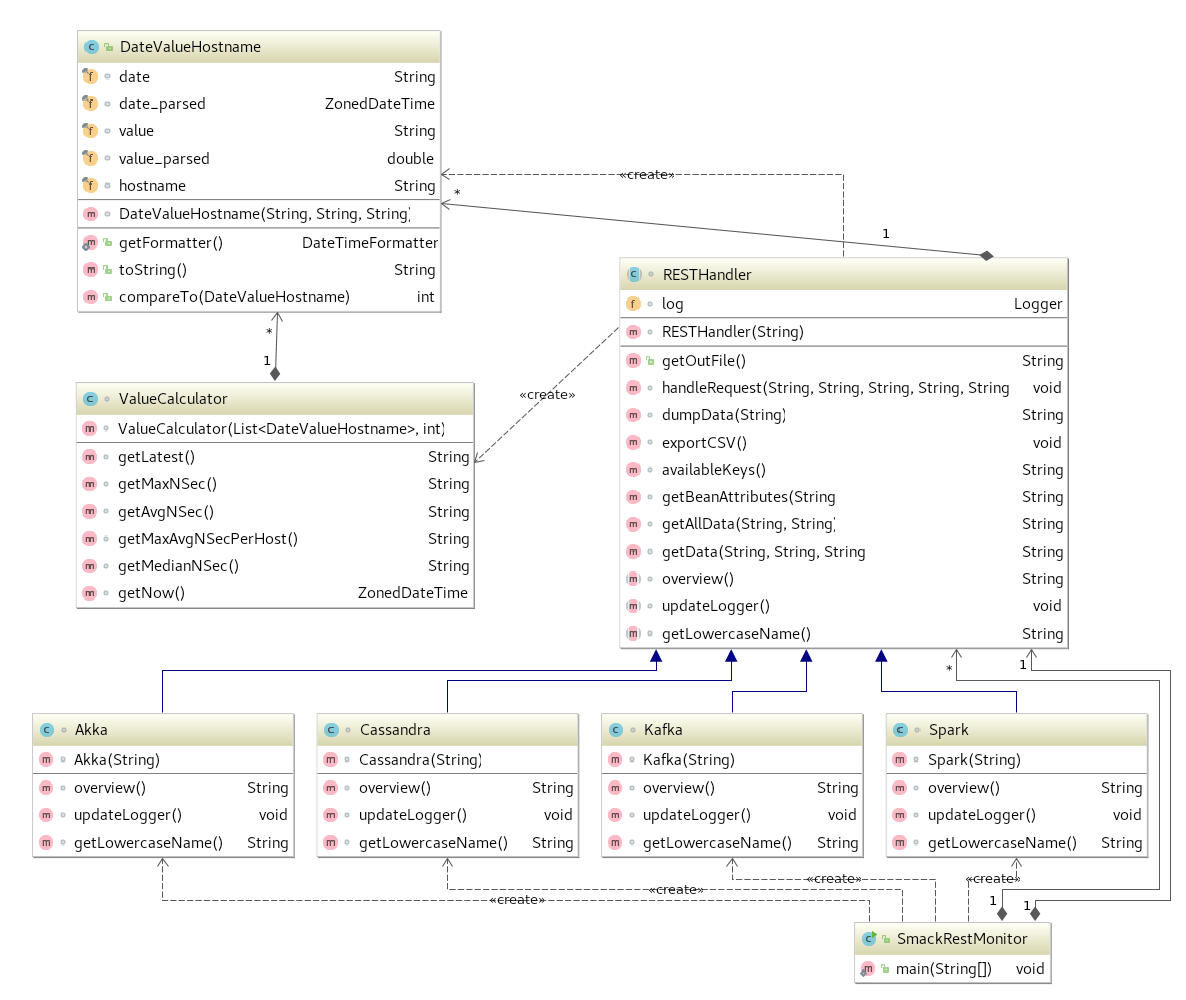
\includegraphics[keepaspectratio=true,scale=0.42]{img/smack_rest_monitor_uml}
    \caption{SMACK REST Monitoring Service}
  \label{fig:smack_rest_monitor_uml}
\end{figure}

\begin{table}[]
\setlength{\extrarowheight}{.5em}
\begin{tabular}{@{}lp{8cm}@{}}
\toprule
URL & Description \\ \midrule
/                                       & Displays an overview page with links to the particular services and available operations.  \\
/<service>                              & Overview page of the respective service which contains links to further operations. \\
/<service>/dump                         & Outputs all stored data associated with the given service. This call is useful for debugging purpose. \\
/<service>/export                       & Returns a properly formatted CSV file containing all collected data of the respective service. \\
/<service>/availableKeys                & Outputs a list of all collected MBeans of a service. \\
/<service>/availableAttributes/:bean    & Generates a list of all available attributes associated with an MBean and a service. \\
/<service>/get/:bean/:attribute         & Displays a new-line separated list of entries of a given service, MBean and attribute from all hosts from the beginning of time. \\
/<service>/get/:bean/:attribute/:value  & The \textit{:value} part of the URL can be one of the following: \newline
                                          \verb|LATEST| Returns the most recent value which is received by the REST service. \newline
                                          \verb|MAX_60_SEC| Calculates the maximum of all hosts for the given MBean / attribute combination during the last 60 seconds. \newline
                                          \verb|AVG_60_SEC| Same as max, but calculates the average. \newline
                                          \verb|MEDIAN_60_SEC| Same as max, but calculates the median. \newline
                                          \verb|MAX_AVG_60_SEC_PER_HOST| Calculates the average of the value for the MBean / attribute combination during the last 60 seconds separately for each available host and returns the maximum value of those averages. \\
/generatePlots                          & Generates plots of all services and all MBeans.
                                          As the generation of the plots is quite computation intense, this action has to be called manually.
                                          The plots are then exposed via the webservice with a simple HTML page containing a list of all available SVG images.\\
\bottomrule
\end{tabular}
\centering
\caption{SMACK REST Monitoring Service API}
\label{tab:rest}
\end{table}




\subsection{Scaling Service}
The tool introduced in this section is responsible for scaling up and down the individual components of the SMACK stack with respect to their utilization.\\
There are defined thresholds for each SMACK component which are observed via the REST monitoring service.
With periodical checks, the latest values are requested from the SMACK monitoring service, introduced in the previous section, and compared against the predefined values.\\
There are two modes: The fully automatic and the suggestive one.
While the tool performs the scaling autonomously in the automatic mode, in the suggestive mode the user can decide whether or not to scale up or down a service based on suggestions.
If a value exceeds the limit, the upscaling action is executed.
Once this has been done, the tool waits for a defined period of time to apply further upscaling to the same service.
Empirical experiments showed, that values under three minutes are too short, as the system takes some time to launch a new instance of the respective component and redistribute the data and workload across the cluster.\\

In Figure~\ref{fig:smack_controller_uml} a UML diagram shows how the tool is designed.
As it can be seen the abstract Service is extended by the respective services, which provide their own implementations of scaling up or down.
In addition the services contain the respective thresholds and URLs to access for the desired values.\\
The Service class provides some utility methods to easily interact with the Marathon environment running under DC/OS, which is responsible for scaling and scheduling services.\\
In Util, some generic helper methods can be found, like executing a command or performing an HTTP GET request.
As expected, ServiceWithUrl is a three-tuple of a service (name), URL and the JMX MBean to query.
This tuple is stored together with a threshold which is then compared against the current values.\\
The central part of this tool is the Controller class, which performs the initial setup and contains the logic needed to perform HTTP requests and asking the services if an action is needed.
Further the management of the timeouts and the interaction with the user is performed in this class.\\

This tool is designed to be executed on a local machine but could be deployed to the cloud as well if needed.
A requirement to successfully scale up and down is the possibility to interact somehow with DC/OS.
In this implementation, the DC/OS command line is used for this purpose and called directly from Java.\\
The user has to install the command line tools provided by DC/OS and has to connect with the stack before running the automated scaling tool.
It would also be possible to use the available REST API, but in this case an authentication would have to be performed additionally by the tool.
In addition the command line provides handy commands which don't come with the REST API.
Due to the generic design of the abstract Service class, the interaction with the stack could be exchanged in just one place without any effort to adapt the services themselves.

\begin{figure}[!htbp]
  \centering
  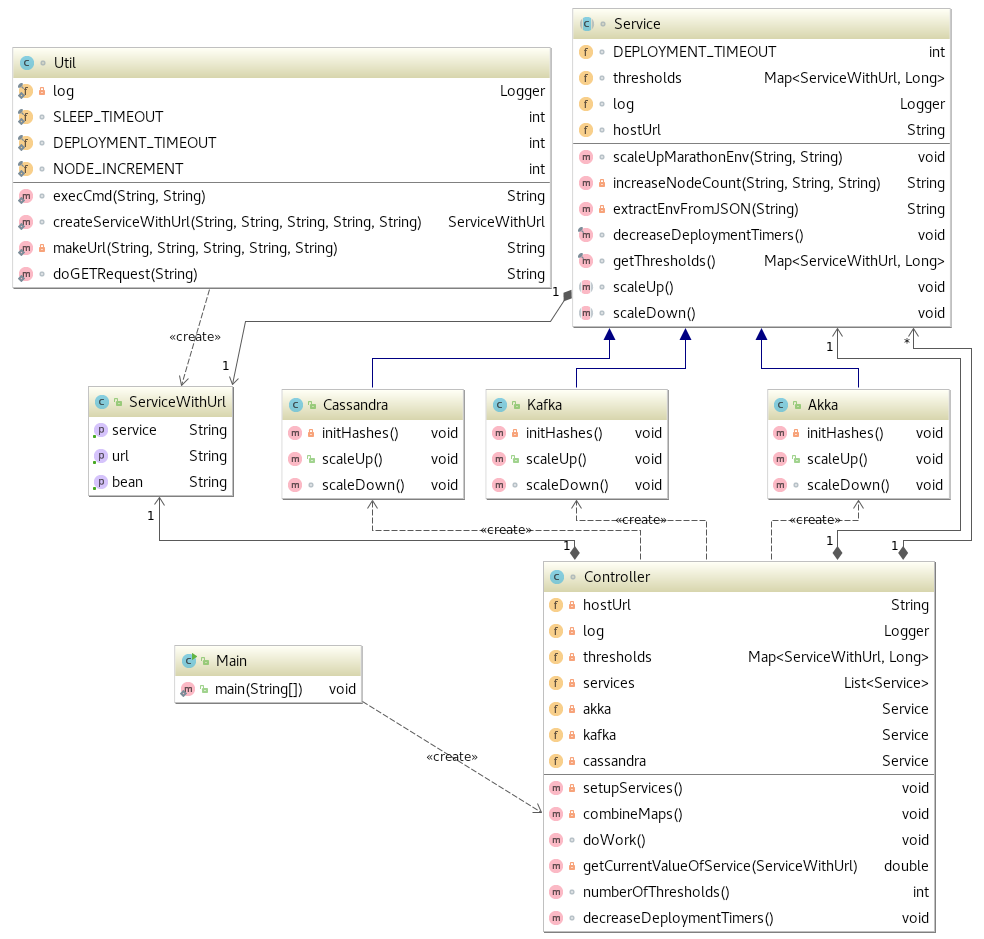
\includegraphics[keepaspectratio=true,scale=0.45]{img/smack_controller_uml}
    \caption{SMACK Controller}
    \label{fig:smack_controller_uml}
\end{figure}



\section{Framework Management Tools and Predefined Blueprints}
The launching and facilitating of a big data stack can get complex and thus automated deployments can help to minimize setup pitfalls.
This section introduces a management tool to quickly deploy the SMACK stack in the cloud, as well as configuration blueprints.

\subsection{Launching Tool}
Launching and setting up a Big Data stack with a cluster abstraction in the cloud is for sure not a trivial task.
To dramatically reduce the manual effort, in the course of this thesis, some tools are used which are described in this section.
AWS provides a Cloud Formation (CF) service, which enables the user to create templates of cloud deployments.
Any kind of AWS resource can be instantiated, configured, mounted or terminated in the template.
It helps system administrators and developers to easily setup a desired running configuration with a few clicks.\\
The CF templates are simple JSON files, which can be created by copying a template from AWS or using the AWS CF template online editor.
A benefit of using CF is that it is also possible to update running stacks, like adding additional nodes etc.
This requires no special update flag, but only the upload of the existing template with the updated values and AWS CF automatically recognizes what has changed and accordingly updates the instances.\\

In this thesis DC/OS (DataCenter OperatingSystem) \cite{dcos}, is used to run the SMACK stack in the cloud.
It is basically an open source, distributed operating system which uses Mesos as its system kernel.
The advantage to use DC/OS is that it leverages the setup of Mesos on multiple nodes and joining them together to one cluster.
In addition there are application packages available for most big data frameworks.
This means, once it is set up, installing Apache Spark is just as much as selecting the package and clicking on install.
DC/OS takes care of launching everything, opening ports, registering nodes etc.\\

Fortunately there is a predefined AWS Cloud Formation template available to launch DC/OS in the cloud offered by DC/OS itself.
Zuehlke Engineering AG provides a repository \cite{shmack} with some handy tools to even more automate the launch of the stack.
The repository offers a configuration file with which all necessary AWS launch parameters can be set and additional bash scripts to gather information once the stack is up and running.\\
As part of this thesis, the used version of DC/OS is updated and several additional helper scripts are provided.
This includes a command to deploy all SMACK components and further install the desired application itself into the stack.
To help new users get into deeper understanding and avoid starting problems, the respective documentation has been updated.


\subsection{Blueprints}
As part of the contribution, reference deployment architecture and configuration, or simply deployment blueprints are produced.
This information is the result of experimenting with resource distribution and scaling up and down services.
The blueprints are given for two kinds of applications running in the SMACK stack, I/O and computational bound.
It is therefore as good entry point when setting up the stack initially, without having to bother with experimenting on how to distribute the resources ideally.\\
During the experiments with the applications described in Section~\ref{sec:iot_application} and Section~\ref{sec:computation_application}, the resource workload is evaluated and based on that results, the deployment architecture and configurations are deduced.
It can be especially useful to have these configurations, if one does not have a lot of experience with the SMACK stack, but still wants to get the most out of the provided resources.\\

In Table~\ref{tab:blueprint-io} the recommended distribution of CPU and RAM for the respective frameworks is listed for a typical I/O intense application, assuming that Akka serves as data ingestion point.\\
Obviously Mesos is not part of the table, as it is the resource manager.
Akka has to handle a lot of requests, which justifies that it gets the most resources.
Depending on how much logic the ingestion application has to perform, CPU is slightly more important than just a lot a memory.\\
Cassandra is in the end of the data pipeline and uses mainly disk storage.
Still this has shown to be sufficient for writing a lot of data, especially because of the master-less and redundant design of Cassandra.\\
Kafka has to handle lots of pre-processed data and - depending on how many consumers there are - needs to stream data to many nodes.
This requires computational power as well as enough memory to be performant and not being the bottleneck.\\
In this context, Spark as the computation engine of the data pipeline, does not have to do a lot of heavy number crunching, but still relies - per design - on enough memory to perform well.\\


Table~\ref{tab:blueprint-computational} gives the recommendation of how to initially launch a computational bound application within the SMACK stack.\\
In this scenario the data ingestion with Akka does not require many resources as there will not be many connections to handle.
Also Kafka will not be under a lot of stress as a consequence.\\
The most work will be done by Spark when performing the heavy computations.
In this case, enough resources are a good idea so that Spark can spawn enough executors and allow those to perform in-memory computations.\\
The recommendation is also to give Cassandra slightly more resources than in the previous setup, as Spark will have to communicate a lot with the database.

\begin{table}[]
\begin{tabular}{lrrr}
\toprule
                   & \textbf{CPU} & \textbf{RAM} \\ \midrule
\textbf{Akka}      & 35\%         & 30\%  \\
\textbf{Cassandra} & 15\%         & 10\%  \\
\textbf{Kafka}     & 35\%         & 35\%  \\
\textbf{Spark}     & 15\%         & 25\%  \\
\bottomrule
\end{tabular}
\centering
\caption{Deployment Blueprint: I/O Bound Application}
\label{tab:blueprint-io}
\end{table}


\begin{table}[]
\begin{tabular}{lrrr}
\toprule
                   & \textbf{CPU} & \textbf{RAM} \\ \midrule
\textbf{Akka}      & 10\%         & 10\%  \\
\textbf{Cassandra} & 25\%         & 25\%  \\
\textbf{Kafka}     & 15\%         & 15\%  \\
\textbf{Spark}     & 50\%         & 50\%  \\
\bottomrule
\end{tabular}
\centering
\caption{Deployment Blueprint: Computational Bound Application}
\label{tab:blueprint-computational}
\end{table}

